\chapter{USE Questionnaire}\label{apendixb}

\small
\textbf{Usefulness}
\begin{itemize}
\item It helps me be more effective.
\item It helps me be more productive.
\item It is useful.
\item It gives me more control over the activities in my life.
\item It makes the things I want to accomplish easier to get done.
\item It saves me time when I use it.
\item It meets my needs.
\item It does everything I would expect it to do.
\end{itemize}
\small
\textbf{Ease of Use}
\begin{itemize}
\item It is easy to use.
\item It is simple to use.
\item It is user friendly.
\item It requires the fewest steps possible to accomplish what I want to do with it.
\item It is flexible.
\item Using it is effortless.
\item I can use it without written instructions.
\item I don't notice any inconsistencies as I use it.
\item Both occasional and regular users would like it.
\item I can recover from mistakes quickly and easily.
\item I can use it successfully every time.
\end{itemize}
\small
\textbf{Ease of Learning}
\begin{itemize}
\item I learned to use it quickly.
\item I easily remember how to use it. • It is easy to learn to use it.
\item I quickly became skillful with it.
\end{itemize}
\small
\textbf{Satisfaction}
\begin{itemize}
\item I am satisfied with it.
\item I would recommend it to a friend. 
\item It is fun to use.
\item It works the way I want it to work.
\item It is wonderful.
\item I feel I need to have it.
\item It is pleasant to use.
\end{itemize}
\small

\textit{Source: From the work of Lund (2001).}
Note: Users rate agreement with these statements on a 7-point Likert
scale, ranging from strongly disagree to strongly agree. Statements in
italics were found to weight less heavily than the others.


% \begin{figure*}
% %\captionsetup{justification=centering,margin=0cm}
% \centering
% 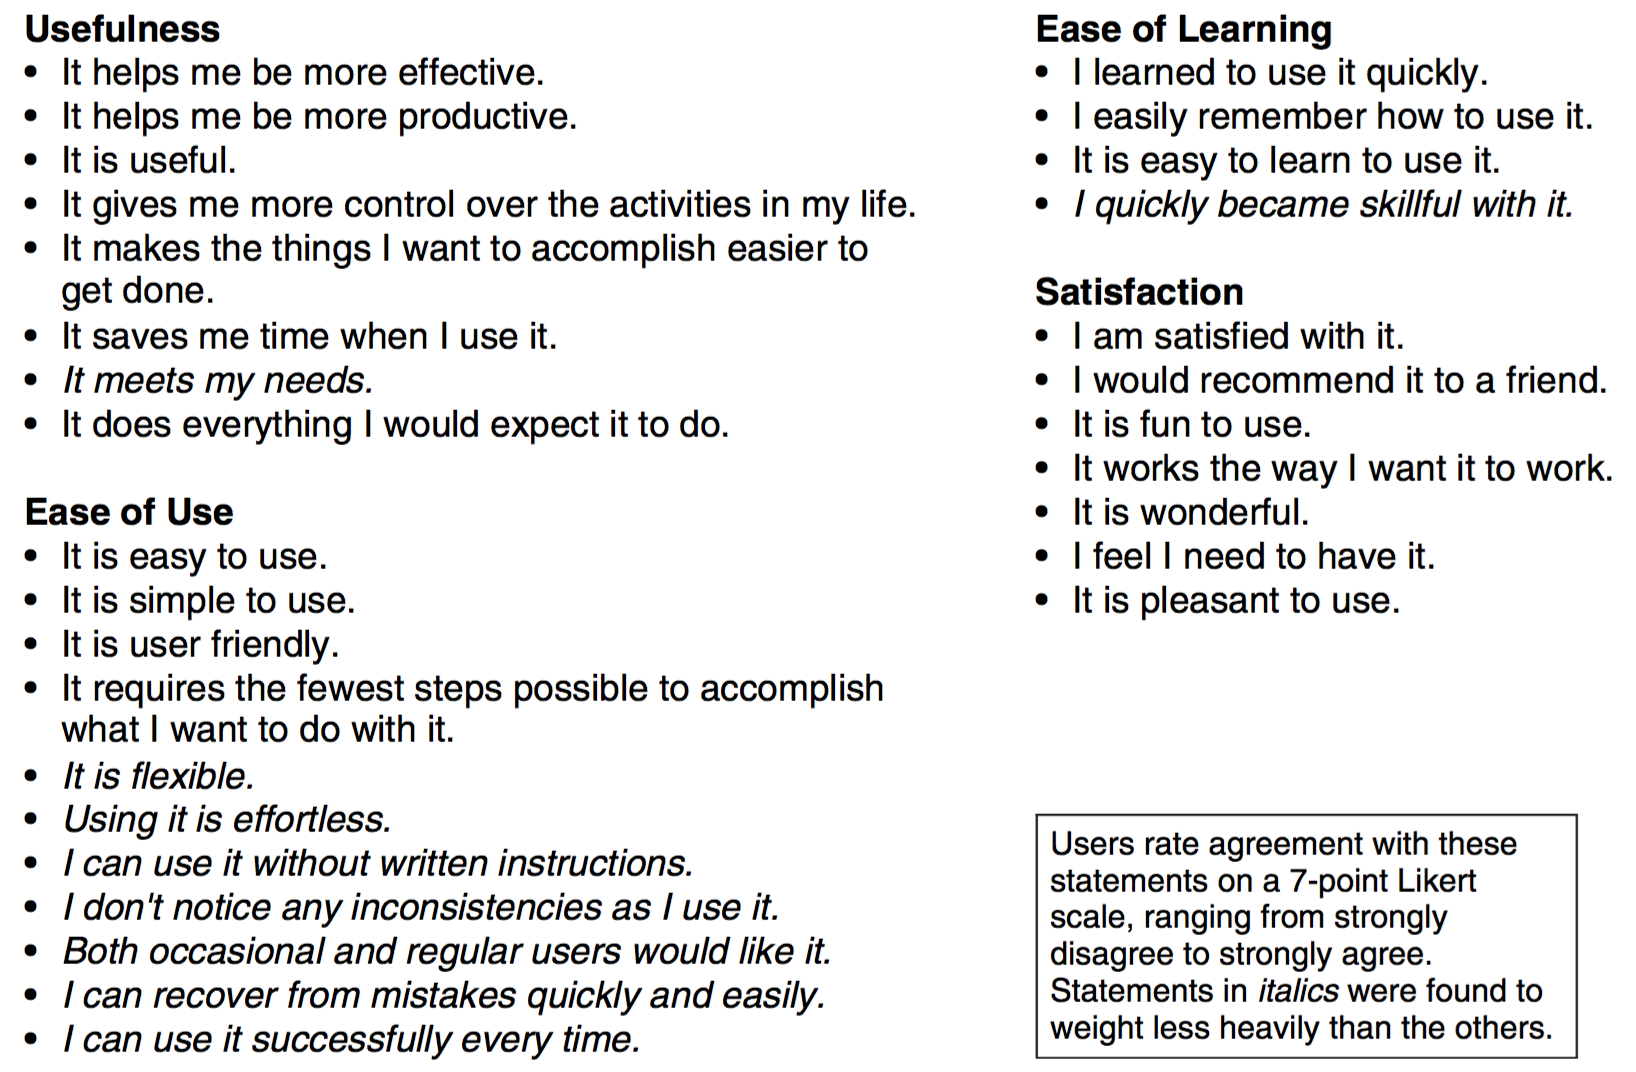
\includegraphics[width=0.5\textwidth]{img/use.png}
% %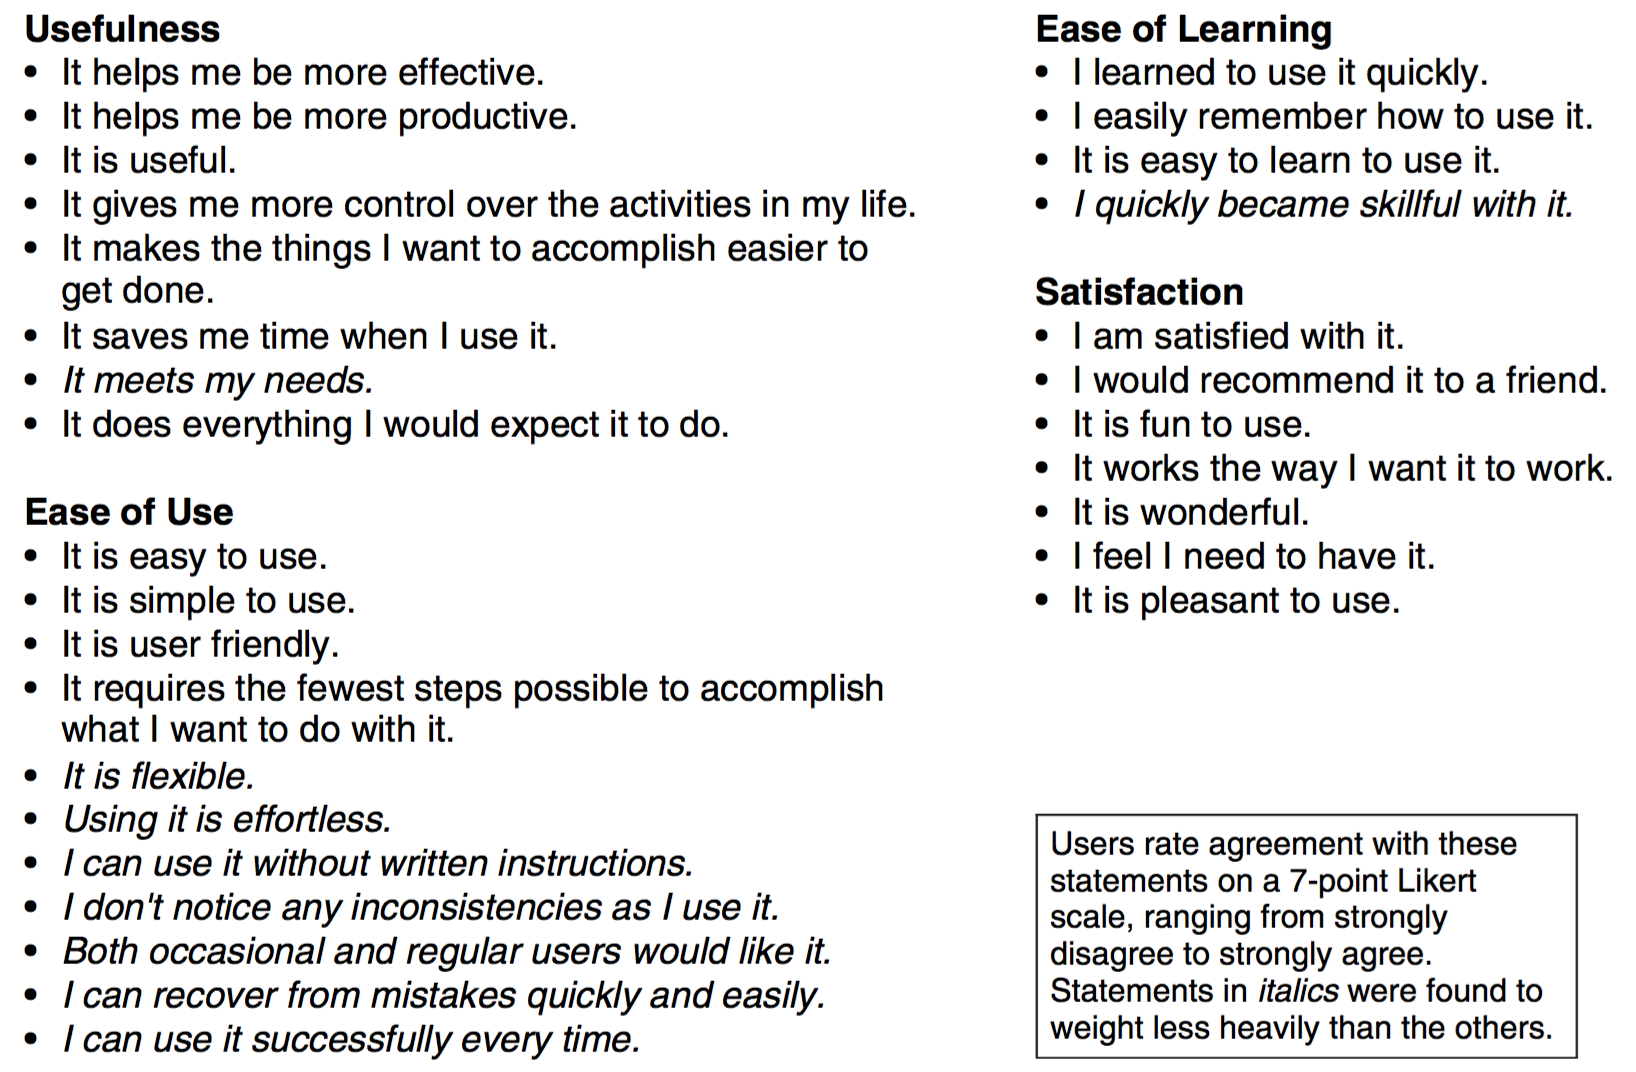
\includegraphics[scale=0.5]{img/use.png} %[width=0.7\textwidth]
% \caption{USE questionnaire.}
% \label{fig:radial}   
% \end{figure*}


% \begin{table}
% \centering
% \tiny
% \caption{USE questionnaire }
% \label{tab:use}      
% \begin{tabular}{p{4cm} p{4cm} }%{ll}
% \hline\noalign{\smallskip}
% Usefulness & Easy of learning  \\
% \noalign{\smallskip}\hline\noalign{\smallskip}
% It helps me be more effective. & I learned to use it quickly.\\
% It helps me be more productive. & I easily remember how to use it. \\
% It meets my needs. & I quickly became skillful with it.\\
% It is useful. &  It is easy to learn to use it. \\
% It gives me more control over the activities in my life.&  \\
% It makes the things I want to accomplish easier to
% get done. & \\
% It saves me time when I use it.  & \\
% It does everything I would expect it to do. &  \\
% \noalign{\smallskip}\hline
% \end{tabular}
% \end{table}

% \begin{table}
% \centering
% \tiny
% \caption{USE questionnaire }
% \label{tab:use}      
% \begin{tabular}{p{4cm} p{4cm} }%{ll}
% \hline\noalign{\smallskip}
% \hline\noalign{\smallskip}
% Easy of use  & Satisfaction \\
% \noalign{\smallskip}\hline\noalign{\smallskip}
% It is easy to use. & I am satisfied with it.\\
% It is simple to use. & I would recommend it to a friend. \\
% It is user friendly. & It is fun to use.\\
% It is flexible. & It works the way I want it to work. \\
% Using it is effortless. & I feel I need to have it.\\
% I can use it without written instructions.& It is wonderful.\\
% I can use it successfully every time. & It is pleasant to use.\\
% It requires the fewest steps possible to accomplish
% what I want to do with it.& \\
% I don't notice any inconsistencies as I use it. &\\
% Both occasional and regular users would like it.& \\
% I can recover from mistakes quickly and easily. &\\
% \noalign{\smallskip}\hline
% \end{tabular}
% \end{table}


















